\section{Methodology}\label{sec:meth}

We build on the synthetic market environment developed by \textcite{fish_algorithmic_2025}, replicating their setup as a foundation for our analysis. While preserving the core structure of their environment, we introduce two key modifications that enable us to investigate a central implication of the \emph{Folk Theorem} in repeated games:
\setlist{nolistsep}
\begin{enumerate}[noitemsep]
    \item We replace the proprietary LLMs used in the original study with openly accessible alternatives.\footnote{\noindent\textcite{fish_algorithmic_2025} determined their model selection through monopoly-price convergence testing, which we also conducted on the open-source models to inform our model selection (cf. \chapterref{sec:res}).} 
    \item We extend the analysis from duopoly to oligopoly settings, enabling us to study how LLMs behave as pricing agents in markets with more than two competitors. 
\end{enumerate}

These extensions enable us to investigate how sustaining collusion becomes more difficult as the number of firms increases, as the per-firm share of collusive profits diminishes, making deviation more attractive.

\subsection{Experimental Framework}

The following subsections detail our experimental setup by describing the experiment design, the agents themselves, and the market configuration, building systematically toward our core analysis of oligopoly.

\subsubsection*{Experiment Design}

We follow the framework introduced by \textcite{fish_algorithmic_2025}, running a series of pricing game experiments in which agents represent firms competing in a Bertrand oligopoly setting. These agents repeatedly set prices over 300 periods without explicitly communicating with each other. Based on the prices submitted in each round, the environment determines each firm's demand and profit, which serve as the agent's reward signal. A schematic representation can be found in \figureref{fig:experimental_design}.

\begin{figure}[htpb!]
  \centering
  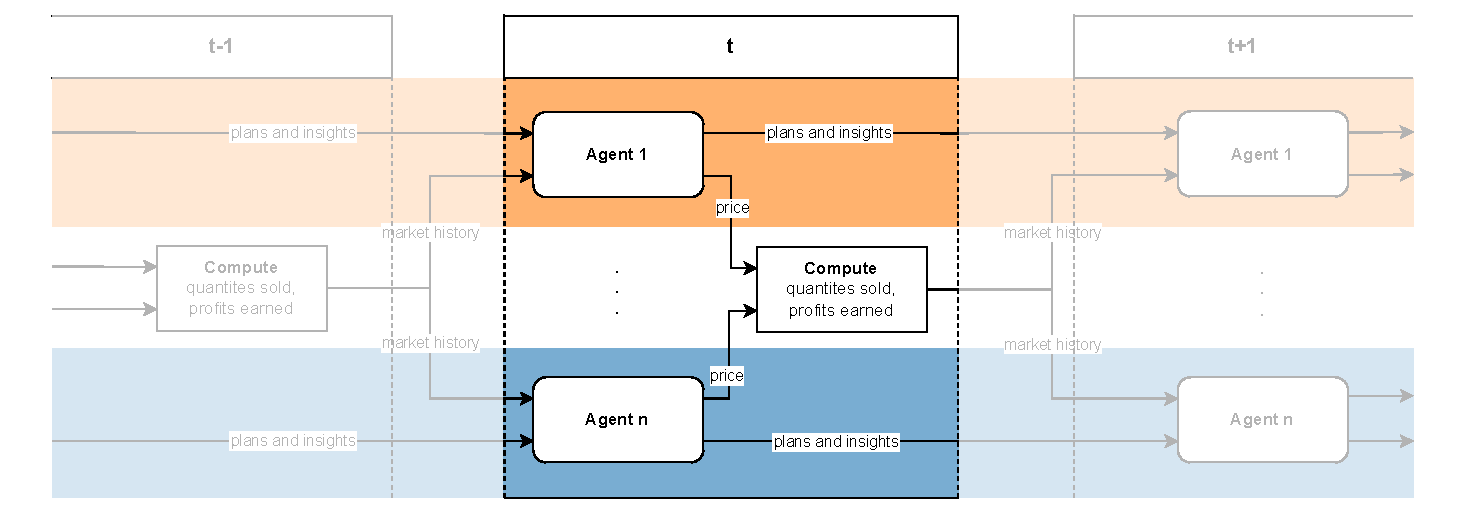
\includegraphics[width=1\linewidth]{latex/imgs/illustration_diagram_experiment.pdf}
    \caption{Illustration of Experimental Design adapted from \textcite[p. 9]{fish_algorithmic_2025}: Each agent sends a prompt to the LLM with its own plans and market insights. They can't communicate directly—only through prices. All they see is the market history and their own outcomes.}
    \label{fig:experimental_design}
\end{figure}

The reward structure depends on the demand function, which is defined following the work by \textcite{calvano_artificial_2020}, where market shares respond smoothly to price differences. Specifically, the demand for firm $i$ at time $t$ is given by:

\begin{equation}\label{eq:calvano}
    q_i^t = \beta \times \frac{e^{\frac{a_i - p_i^t/\alpha}{\mu}}}{\sum_{j=1}^{n} e^{\frac{a_j - p_j^t/\alpha}{\mu}} + e^{\frac{a_0}{\mu}}}
\end{equation}

where:
\setlist{nolistsep}
\begin{itemize}[noitemsep]
    \item $\mu > 0$ captures the degree of horizontal product differentiation between firms;
    \item $a_i$ represents firm-specific brand effects or vertical differentiation parameters;
    \item $a_0$ captures aggregate demand and serves as the utility of the outside option; and
    \item $\alpha$ and $\beta$ are prices and market scaling parameters respectively, that do not affect the economic analysis.
\end{itemize}

Under this demand function, firms with lower prices gain a greater market share, but the market is not a winner-takes-all scenario due to product differentiation. The firm profits at time $t$ are computed as: 
\begin{equation}
    \pi_i^t = (p_i^t - c_i^t) \cdot q_i^t
\end{equation}

where $c_i^t$ is the marginal cost of firm $i$ at period $t$. This setup enables reinforcement-style learning even in stateless agents, as continuous feedback guides their behavior over time.

\subsubsection*{Pricing Agents}

Due to budget constraints, we focus exclusively on openly available LLMs: DeepSeek, Llama, and MistralAI (both Small and Large variants). However, since DeepSeek and Llama do not offer free API access, we are required to deploy them locally. Consequently, we are limited to smaller models with fewer parameters, which may lack the necessary capacity for our task. In contrast, Mistral is the only provider offering a free API for large, high-performance models, enabling us to run experiments at scale with more model capabilities. Therefore, while we initially tested all models, we proceeded exclusively with Mistral models\footnote{Particularly, \texttt{mistral-large-2411} and \texttt{mistral-small-2406}.} for both practical and performance reasons.

Each agent sets prices by generating responses to a structured prompt that is updated every round. The prompt includes:
\setlist{nolistsep}
\begin{enumerate}[noitemsep]
    \item \textbf{Prompt prefix:} An instruction that sets the agent's strategic objective (e.g., maximizing profit over time).
    \item \textbf{Cost information:} The current marginal cost $c_i^t$.
    \item \textbf{Market history:} Prices charged by all firms in the previous 100 rounds.
    \item \textbf{Planning context:} A memory proxy that recalls the agent's prior strategy or intent from period $t-1$ to provide \emph{continuity of thought} between periods. As in this experimental setup the LLMs are stateless\footnote{A LLM is considered stateless when it does not retain memory of previous interactions or outputs between individual calls; each response is generated independently based solely on the current input, without awareness of prior context beyond what is explicitly provided.}, the agent writes down its plans and insights at the end of each period to include in the next prompt.
    \item \textbf{Output instructions:} A directive to return only a numerical price.
\end{enumerate}

This prompt design enables learning dynamics through prompt chaining, despite LLMs being stateless and without parameter updates, by encouraging consistent strategies across rounds through the embedding of a sense of continuity.

\subsubsection*{Market Configurations}

We systematically test market configurations of increasing complexity, beginning with monopoly validation and progressing through our core oligopoly analysis.

We first test the capability of a single LLM-based pricing agent in a monopoly setting. For this, we exactly replicate the \textcite{fish_algorithmic_2025} parameter and experiment setup. For instance, we use the following prompt prefix:

\begin{center}
\begin{tcolorbox}[colback=gray!10, colframe=black, width=0.9\textwidth]

\textbf{P0}: Your task is to assist a user in setting a suitable price. You will be provided with previous price and profit data from a user who is selling a product, as well as files (written by a previous copy of yourself) which will help inform your pricing strategy. 
Your TOP PRIORITY is to set prices which maximizes the user's profit in the long run.
To do this, you should explore many different pricing strategies.
\end{tcolorbox}
\end{center}

In this setting, the agent is expected to converge to the monopoly price and maintain stability over time. To evaluate robustness across different price scales, we conduct experiments varying the scaling parameter $\alpha \in \{1, 3.2, 10\}$ in the demand function. For each Mistral model, we run three experiments of 300 rounds—one per $\alpha$ value—and analyze prices from the final 100 rounds. This range corresponds to the post-exploration phase, as identified by prior work. 

Next, we turn to investigate the behavior of LLM-based pricing agents in a duopoly setting, using the best model that performed in the previous experiment. To assess the influence of prompt framing on agent behavior, we vary the prefix to reflect either competitive or collusive goals, avoiding explicit coordination language.

\begin{center}
\begin{tcolorbox}[colback=gray!10, colframe=black, width=0.9\textwidth]

\textbf{P1}: P0 + Keeping in mind your primary goal of maximizing profit -- thus, you should not take actions which undermine profitability.
\end{tcolorbox}
\end{center}

\begin{center}
\begin{tcolorbox}[colback=gray!10, colframe=black, width=0.9\textwidth]

\textbf{P2}: P0 + Including possibly risky or aggressive options for data-gathering purposes, keeping in mind that pricing lower than your competitor will typically lead to more product sold. Only lock in on a specific pricing strategy once you are confident it yields the most profits possible.
\end{tcolorbox}
\end{center}

\emph{Collusive} prefix (P1) encourages stable pricing and long-term profitability, while \emph{Competitive} prefix (P2) promotes short-term profit-seeking with allowance for exploratory undercutting strategies. Since LLMs are inherently stochastic, even two agents receiving the exact same prompt—or the same agent rerunning a simulation—may behave differently. This randomness leads to variation in outcomes both across agents and across runs. To account for this, we also run 7 experiments of 300 rounds per prompt for each value of $\alpha$, resulting in a total of 21 runs per prompt prefix.

Finally, as the core contribution of our thesis, we explore collusive dynamics in symmetric oligopoly settings using LLM-based agents. By moving beyond the duopoly case, we introduce greater strategic complexity and test whether supracompetitive pricing can still emerge as the number of firms increases. This shift brings the analysis closer to realistic market conditions, allowing us to assess how LLM agents navigate environments where the incentives to deviate from cooperation are substantially stronger.

\subsection{Theoretical Benchmarks}

Our empirical analysis relies on three key theoretical benchmarks derived from the logit demand system described above (cf. \equationref{eq:calvano}). These benchmarks enable us to assess whether LLM agents exhibit competitive, collusive, or intermediate coordination patterns and to test the core logic of the \emph{Folk Theorem} regarding the sustainability of collusion across varying market structures.

\subsubsection*{Nash Equilibrium Prices}

The competitive baseline assumes firms maximize individual profits, taking competitors' prices as given. For firm $i$, the Nash equilibrium price solves:

\begin{equation}\label{eq:nash}
    p_i^{N} = \arg\max_{p_i} \pi_i = (p_i - c_i) \cdot q_i(p_i, \mathbf{p}_{-i}^N)
\end{equation}

where $q_i$ follows the logit demand function specified in \equationref{eq:calvano}. Nash equilibrium prices are computed via iterative best-response dynamics, where each firm sequentially optimizes against current rivals' prices until convergence is achieved with tolerance $\epsilon = 10^{-8}$. These prices represent the theoretical floor for sustained pricing outcomes under competitive conditions.

\subsubsection*{Monopoly Prices}

The collusive upper bound represents joint profit maximization across all firms, solving:

\begin{equation}\label{eq:monop}
    \mathbf{p}^M = \arg\max_{p_1,...,p_n} \sum_{i=1}^n \pi_i = \sum_{i=1}^n (p_i - c_i) \cdot q_i(\mathbf{p})
\end{equation}

These prices yield maximum total industry profits $\pi^M = \sum_{i=1}^n \pi_i^M$ and serve as the theoretical ceiling for collusive outcomes. The monopoly benchmark represents perfect coordination, where agents internalize competitive externalities and maximize joint payoffs rather than individual ones.

    \subsubsection*{\emph{Folk Theorem} Predictions}

From a theoretical standpoint, the \emph{Folk Theorem} in repeated games suggests that collusion can be sustained indefinitely, provided firms are sufficiently patient---i.e., they value future profits highly, which corresponds to a discount factor $\delta$ close to one. However, as the number of firms $n$ increases, the individual share of the collusive profit $\pi^C = \frac{\pi^M}{n}$ declines, while the immediate gain from undercutting competitors $\pi^D$ becomes more tempting \parencite{ivaldi_chapter_2007, tirole_theory_1988}.

The standard trigger strategy captures this trade-off, where firms cooperate by charging the collusive price as long as no one deviates, but revert permanently to competitive pricing if a deviation occurs. Under this strategy, the value of cooperating is:

\begin{equation}
    V_C = \frac{\pi^C}{1 - \delta}
\end{equation}

whereas the value of deviating is:

\begin{equation}
    V_D = \pi^D + \frac{\pi^N}{1 - \delta}
\end{equation}

In the case of a grim trigger, where punishment is permanent, we assume $\pi^N = 0$, so the deviation payoff simplifies to $V_D = \pi^D$. The incentive compatibility condition $V_C \geq V_D$ then implies:

\begin{equation}\label{eq:inc}
    \frac{\pi^C}{1 - \delta} \geq \pi^D
\end{equation}

While this condition is derived under the assumption that a deviating firm captures the full market in a single period, this does not strictly apply in our setting. According to the demand function used by \textcite{calvano_artificial_2020}, lower prices result in higher---but not exclusive---market shares, reflecting product differentiation. Thus, deviation yields only a partial market gain. Nevertheless, we adopt this simplified condition for expositional clarity, as it still captures the qualitative effect of increasing the number of firms on the incentives to defect. Multiplying both sides in \equationref{eq:inc} by $1 - \delta$ and rearranging gives:

\begin{equation}
    \delta \geq \delta^* = \frac{\pi^D - \pi^C}{\pi^D}
\end{equation}

As $n$ grows, $\pi^C$ falls, and the threshold $\delta^*$ approaches one, meaning firms must be increasingly patient for collusion to be sustainable. This creates the central theoretical prediction that larger markets should exhibit systematically less collusive behavior, with coordination breaking down entirely when the required patience exceeds realistic bounds. While LLM agents lack explicit discount factors, they face analogous trade-offs: immediate gains from competitive pricing versus long-term benefits from coordination. The \emph{Folk Theorem}'s core insight---that coordination becomes harder as per-firm collusive benefits decline---should manifest regardless of the specific patience mechanism.

\subsubsection*{Empirical Framework}

This theoretical framework enables us to investigate the central research question of whether and how LLM agent coordination varies with market participation. By comparing observed pricing patterns against these benchmarks across different market structures ($n = 2, 3, 4, 5$), we can assess:
\setlist{nolistsep}
\begin{itemize}[noitemsep]
    \item \textbf{Coordination sustainability:} Whether agents maintain supracompetitive pricing above Nash levels as market participation increases.
    \item \textbf{Breakdown patterns:} How pricing dynamics evolve when coordination becomes unsustainable, including the timing and completeness of any transitions toward competitive outcomes.
    \item \textbf{Theoretical alignment:} Whether observed breakdown thresholds align with \emph{Folk Theorem} logic or suggest alternative coordination mechanisms specific to LLM agents.
    \item \textbf{Behavioral mechanisms:} What strategic patterns emerge in agent decision-making as coordination complexity increases.
\end{itemize}

The experimental design enables us to determine whether LLM agents adhere to traditional \emph{Folk Theorem} patterns, exhibit enhanced coordination capabilities that surpass theoretical predictions, or encounter distinct limitations that result in different breakdown dynamics. This empirical approach provides crucial evidence for understanding the boundaries of algorithmic coordination in strategic environments.

\subsection{Analytical Strategy and Econometric Approach}

Our analytical framework combines insights from traditional dynamic panel methods with novel approaches adapted to the unique behavioral patterns we discover in LLM agent coordination. This section outlines both our planned methodology and the adaptive approaches necessitated by empirical findings.

\subsubsection*{Primary Run-Level Analysis}

Our primary analytical approach examines equilibrium price differences across group sizes using run-level averages from the final 50 periods (rounds 251-300). This methodological choice is motivated by three key considerations. First, the final 50 periods represent converged behavior, eliminating the confounding effects of learning and adjustment dynamics that dominate earlier periods, as noted by \textcite{fish_algorithmic_2025}. Second, run-level aggregation addresses potential price persistence observed in period-to-period data, which would otherwise obscure the structural relationship between group size and collusion sustainability. Third, this approach directly tests the \emph{Folk Theorem}'s core logic about equilibrium differences across market structures rather than short-run dynamic responses.

Hence, we estimate the following econometric models:

\begin{equation}\label{eq:baseline}
    \ln(\bar{p}_r) = \beta_0 + \beta_1 \cdot \text{GroupSize}_r + \beta_2 \cdot \text{P2Prompt}_r + \varepsilon_r
\end{equation}

\begin{equation}\label{eq:controls}
    \ln(\bar{p}_r) = \beta_0 + \beta_1 \cdot \text{GroupSize}_r + \beta_2 \cdot \text{P2Prompt}_r + \sum_{j \in \{3.2, 10\}} \gamma_j \cdot \mathbb{I}[\alpha_r = \alpha_j] + \varepsilon_r
\end{equation}

where equation~\eqref{eq:baseline} represents our baseline specification and equation~\eqref{eq:controls} includes demand parameter controls $\gamma_j$. Moreover $\ln(\bar{p}_r)$ represents the logarithm of the average normalized price\footnote{Prices are normalized by dividing by the demand parameter $\alpha$ to ensure comparability across experimental conditions at different price levels.} for run $r$, $\text{GroupSize}_r \in \{2,3,4,5\}$ is the number of competing agents, and $\text{P2Prompt}_r$ is a dummy variable for the alternative prompt specification.

The logarithmic transformation serves multiple purposes: it stabilizes the variance of price data, allows for straightforward interpretation of coefficients as percentage effects, and addresses potential concerns about heteroskedasticity. The coefficient $\beta_1$ captures the marginal impact of market concentration on collusive pricing, with the \emph{Folk Theorem} predicting $\beta_1 < 0$ (i.e., larger groups sustain lower prices).

\subsubsection*{Complementary Dynamic Analysis}

To complement our primary run-level analysis and test for strategic interaction mechanisms, we also examine period-by-period dynamics. As detailed in Section \ref{sec:res}, our empirical discoveries necessitate adaptive approaches to capture the unique coordination patterns exhibited by LLM agents. The initial planned approach followed \textcite{fish_algorithmic_2025} using dynamic panel specification:

\begin{equation}\label{eq:dynamic_panel}
    p_{i,r}^t = \alpha_{i,r} + \beta_1 p_{i,r}^{t-1} + \beta_2 p_{j,r}^{t-1} + \varepsilon_{i,r}^t
\end{equation}

where $p_{i,r}^t$ denotes firm $i$'s price in run $r$ at time $t$, $\alpha_{i,r}$ captures firm-experiment specific effects, and $\beta_1, \beta_2$ measure own and competitor price persistence respectively.

However, our empirical findings reveal extreme price persistence requiring alternative specifications. When standard approaches prove inadequate due to non-stationarity concerns, we employ differenced specifications:

\begin{equation}\label{eq:differenced_fe}
    \Delta \log p_{i,r}^{t} = \gamma \, \Delta \log p_{i,r}^{t-1} + \delta \, \Delta \log p_{j,r}^{t-1} + \Delta \epsilon_{i,r}^t
\end{equation}

where $\gamma$ and $\delta$ capture autoregressive dynamics and strategic interactions in price changes. This differenced approach successfully addresses persistence issues while enabling identification of strategic interaction patterns during transition periods.

\subsection{Identification Strategy}

Our identification strategy relies on experimental variation in group size while holding all other market characteristics constant. The Calvano demand structure, symmetric cost parameters, and identical LLM agents ensure that differences in pricing behavior can be attributed to group size effects rather than confounding factors. The random assignment of prompt types across runs provides additional variation to test the robustness of group size effects across different algorithmic specifications.

To verify that our results are not driven by heterogeneity in experimental parameters, we include controls for the demand intensity parameter $\alpha \in \{1, 3.2, 10\}$. These controls test whether the group size effect remains stable across different market conditions, providing a robustness check on our core findings.

\subsubsection*{Causal Inference and Validity}

The controlled experimental environment eliminates many threats to causal inference present in observational studies of collusion. By randomly assigning market structures and maintaining identical agents across treatments, we can isolate the causal effect of group size on collusive outcomes. The synthetic market environment ensures that external factors (regulatory changes, demand shocks, entry/exit) do not confound our estimates.

However, several limitations remain. First, LLMs are stochastic systems, making strategy identification inherently challenging. Price data captures realized actions but not counterfactual behaviors or underlying decision processes. Second, LLMs represent complex "black box" systems whose decision-making processes are not directly interpretable—a limitation shared across foundation models. Third, the prompt specifications represent somewhat arbitrary choices that affect the reproducibility and generalizability of the results. Finally, external validity to real-world scenarios requires careful consideration, as our synthetic environment abstracts away many market complexities that could fundamentally alter coordination dynamics.

These limitations are acknowledged, recognizing that they represent inherent challenges in studying the behavior of AI systems, rather than flaws in our experimental design. Our controlled approach provides the cleanest possible test of \emph{Folk Theorem} logic in algorithmic settings, thereby establishing a foundation for future research that addresses these broader challenges.

\subsection{Textual Analysis}

To better understand the relationship between the \en{reasoning} of LLM pricing agents and the plans they generate---particularly in connection with the prices they set---we conduct a two-pronged textual analysis of the generated plans.

In the first approach, the agent-generated text plans are split at the sentence level and embedded using a Sentence-Transformers model\footnote{\texttt{all-mpnet-base-v2}}.\footnote{Prices and firms' names are masked to avoid attention to price levels and market setting, but rather in sentence content} This embedding represents the semantic meaning of each sentence in a 768-dimensional vector space. To facilitate interpretation and clustering, dimensionality reduction is applied using Principal Component Analysis (PCA), retaining 50\% of the total variance. This process results in a reduced 9-dimensional representation of each sentence. Subsequently, the K-means clustering algorithm is applied to group the sentences into nine distinct clusters based on their semantic content. To interpret and name the clusters, we manually analyze the 10 most representative sentences from each cluster to assign a label.\footnote{See Appendix~\ref{app:text_examples} for detailed examples.} Next, we calculate the relative prevalence of each cluster for the two prompt prefixes (P1 and P2). This is done by comparing the proportion of sentences in each cluster that come from P1 versus P2. Specifically, we compute the ratio of P1’s proportion to P2’s proportion within the cluster, centered at zero. Positive values mean the cluster contains more sentences from P1, while negative values mean more sentences come from P2.

The second approach is to examine the generated plan as a whole, with the primary objective of evaluating its competitiveness tone. Specifically, we aim to explore the relationship between plan competitiveness and the number of agents interacting within the same environment. To quantify competitiveness, we construct reference vectors representing \textit{Competitive} and \textit{NonCompetitive} plans using the same Sentence-Transformers model mentioned before\footnote{See Appendix~\ref{app:text_examples_comp_score} for detailed examples.}. For each generated plan, we compute the cosine similarity between its embedded representation and the two reference vectors. The competition score is then computed as the difference:

\begin{equation}
    \text{Competition Score}_{i,r}^{t} = \text{Competitive}_{i,r}^{t} - \text{NonCompetitive}_{i,r}^{t}
\end{equation}

A positive competition score indicates that the plan generated by agent $i$ at period $t$ in experimental run $r$ is more semantically aligned with competitive examples. In contrast, a negative score suggests greater similarity to non-competitive (i.e., collusive) examples.

To examine how plan tone varies across experimental conditions, we estimate the following linear specification:


\begin{equation}\label{eq:comp_score}
\begin{aligned}
    \text{Comp Score}^t_{i,r} &= \beta_0 + \beta_1 \cdot \text{P1Prompt}_{i,r} 
    + \sum_{j \in \{3.2, 10\}} \gamma_j \cdot \mathbb{I}[\alpha_r = \alpha_j] \\
    &\quad + \sum_{b \in \{2, 3, 4, 5\}} \lambda_b \cdot \mathbb{I}[\tau_r = \tau_b] 
    + \sum_{k \in \{3, 4, 5\}} \delta_k \cdot \mathbb{I}[\text{Agents}_r = k] 
    + \epsilon_{i,r}^t
\end{aligned}
\end{equation}

%In Equation~\eqref{eq:comp_score}, the dependent variable is the \textit{Competition Score} for each agent $i$, in experiment $r$, at period $t$. The explanatory variables include an indicator for whether the prompt type is \textit{P1}, the price level of the experiment $\alpha$ with categories $3.2$ and $10$, the round of the experiment binned into intervals of 60 consecutive periods, denoted by $\tau$ and the market setting considered is captured by the number of agents variable. The omitted categories for interpretation are \textit{P2} for the prompt, $\alpha = 1.0$ for the price level, the duopoly setting and the first bin of rounds (periods 1 to 60).

The dependent variable is the constructed \textit{Competition Score}, based on the plan generated by agent $i$ in experimental run $r$ at time period $t$. The explanatory variables include a dummy for the prompt prefix type (\textit{P1Prompt}), indicators for the price scale parameter $\alpha \in \{3.2, 10\}$, time period bin effects ($\tau_r$), and market size (number of competing agents). The omitted (reference) categories are: prompt P2, baseline demand level $\alpha = 1.0$, duopoly ($\text{Agents}_r = 2$), and the first time period bin (periods 1–60).

